\section{Lithium teknologi}
Lithium batterier har siden 1973 været under konstant udvikling. Gennem tiden er der opdaget mange forskellige typer for lithium batterier. Målet er, som ved så mange andre typer batterier, at få den højeste kapacitet på mindst mulig plads. Men da der ved lithium batterier er farlige konsekvenser ved dette, er man nødt til at finde det bedste kompromis. "Hovednavnet" \space /det mest brugte navn for de mange forskellige typer er bare "lithium-ion" \space men hvis man går lidt dybere ned i kemien ser man at der findes lithium-ion batterier med mange forskellige karakteristika. 

\subsection{Lithium cobalt oxid}
Den nok mest brugte er dog lithium cobalt oxid-typen ($LiCoO_2$) som bruges i f.eks. mobiltelefoner og moderne bærbare computere. Denne type er den mest fleksible i dens fysiske design, men også den farligste. Derfor er det vigtigt at denne type celle har et overvågningskredsløb, da der ellers kan forekomme katastrofale situationer. Disse celler er oftest formet som "bløde puder" \space \textemdash \space altså uden en hård kasse rundt om. Denne teknologi bruges også oftest i lithium ion polymer-varianten, som bliver brugt meget i RC-industrien pga. den høje afladekapacitet. 

\subsection{Lithium jern fosfat og lignende}
Lithium jern fosfat ($LiFePO_4$) har sammen med lithium ion mangan oxid ($LMO$) og lithium nikkel mangan cobalt oxid ($NMC$) en lavere energidensitet men er mere sikker end lithium cobalt oxid. De har også en længere levetid og derfor er de meget brugte i f.eks. elektrisk værktøj eller medicinindustrien. Sidstnævnte ($NMC$) er især dominerende i elektriske biler. Disse celler findes oftest i 18650 varianten, som er en rund cylindrisk celle. Det er også denne type celle der er valgt til dette projekt, da det efterhånden er en ret standard celle, og da dens karakteristika er ganske veldokumenteret. 

\section{Anvendelse}
Den valgte type lithium-ion celle har en nominal spænding på $3.6\volt$. "Sikkerhedszonen" \space anses for at ligge mellem $3\volt$ og $4.2\volt$. Lades cellen til mere end $4.2\volt$ tager cellen skade og mister kapacitet. Det er også over dette niveau at de katastrofale situationer kan finde sted. Det samme gælder for afladningen. Aflades cellen under $3\volt$ går det også ud over kapaciteten men ikke i samme rate. Nogle typer kan også holde til afladning ned til $2.5\volt$, så denne grænse er en smule mere udefineret.\\
\sbf{Redefiner lidt af formuleringen her}

Kigges der på en typisk 18650 celle såsom Samsung 30Q modellen, har den en afladningskurve (ved $5\ampere$) der ser ud som følgende: 

\begin{figure}[h]
\centering
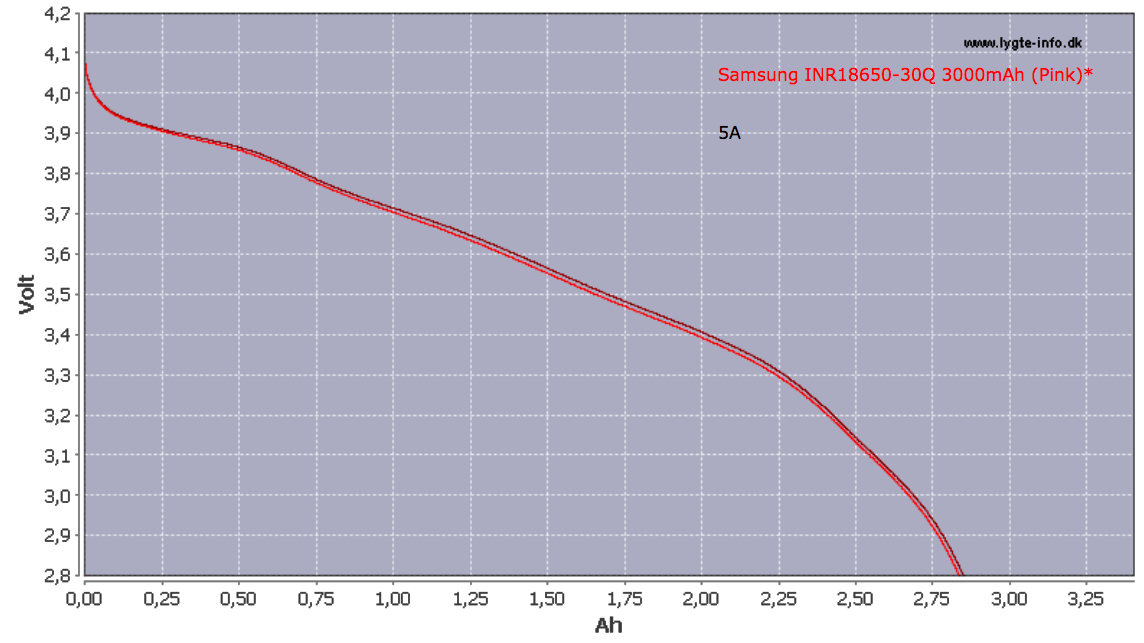
\includegraphics[width=15cm]{billeder/samsung-inr18650-discharge.png}
\caption{Afladekurven for en Samsung INR18650 30Q celle\protect\footnotemark}
\label{fig:30q_discharge}
\end{figure}
\footnotetext{Kurve fra celle-sammenligningsværktøj på Lygte Info's hjemmeside. \url{https://lygte-info.dk/review/batteries2012/Common18650comparator.php}}

Op- og afladning - brugertilpasning (Storage mode etc..)

\section{Sikkerhed}

Kortslutning, overophedning, state of health, afladningsbeskyttelse
